\begin{Ueberlieferung}% 
{\textit{L}}Konzept: LH XXXVII 3 Bl. 86.
1 Bl. 4\textsuperscript{o}, am oberen Rand leicht beschnitten. 2~S.
Ein Wasserzeichen.
\newline%
Cc 2, Nr. 1133 A
\end{Ueberlieferung}
%
%\begin{Datierungsgruende}%
%Von Leibniz datiert.
%\end{Datierungsgruende}
%
\count\Afootins=1200
\count\Bfootins=1200
\count\Cfootins=1200
\pstartfirst
% [86~r\textsuperscript{o}]
[86~r\textsuperscript{o}]%
\textso{ 25 Novemb. 1675.}
Mons. le Duc de Roanez\protect\index{Namenregister}{\textso{Roanez}, Artus Gouffier de 1627-1696} m'a communiqu\'{e} aujourdhuy quelques pensées et observations à l'égard
des eaux courantes. Il \edtext{dit que si de deux rivieres}{\lemma{dit}\Bfootnote{\textit{(1)}\ que les rivieres \textit{(2)}\ que si de deux rivieres \textit{L}}} le penchant est égal, celle qui est la plus profonde sera la plus rapide. Il dit que la Seine est en effect plus rapide que la Loire. Que dans les inondations\protect\index{Sachverzeichnis}{inondation} quand les eaux 
croissent, leur vistesse croist aussi. A Paris\protect\index{Ortsregister}{Paris} du temps de la grande inondation\protect\index{Sachverzeichnis}{inondation}, on fit l'observation suivante, 
on jetta \edtext{un bois}{\lemma{un}\Bfootnote{\textit{(1)}\ poids d \textit{(2)}\ poids \textit{(3)}\ bois \textit{L}}} dans la riviere, avec une fisselle, et on remarqua en combien de temps combien de la fisselle estoit employé. Par apres l'eau n'estant cr\^{u} que de quatre pieds de hauteur d'avantage; on trouua que la vistesse\protect\index{Sachverzeichnis}{} estoit augmentée de plus d'un tiers. L'Hypothese qu'il fait pour expliquer cecy est bien jolie, il dit supposez un canal penchant, dans lequel l'eau coule. Couurez là d'un aix\protect\index{Sachverzeichnis}{aix} long, qu'elle porte. A present imaginez vous que cet aix\protect\index{Sachverzeichnis}{aix} soit recourbé luy m\^{e}me en forme de canal nageant, plein d'autre eau, cette eau qui est dans le canal nageant \edtext{ira d'une vistesse double}{\lemma{ira}\Bfootnote{\textit{(1)}\ du double de la vistesse \textit{(2)}\ d'une vistesse double \textit{L}}} de celle de l'eau qui porte le canal nageant dans le quel elle est; à cause qu'elle va de la vistesse de l'eau\protect\index{Sachverzeichnis}{eau} qui la porte, et encor de la sienne: comme une boule qui roule sur un plan incliné, qui glisse luy m\^{e}me sur un autre plan incliné. Imaginez vous a present que toute la  
\edtext{profondeur de l'eau}{\lemma{profondeur}\Bfootnote{\textit{(1)}\ d'eau \textit{(2)}\ de l'eau \textit{L}}} d'estage en estage soit entrecoupée \edtext{par ces}{\lemma{par}\Bfootnote{\textit{(1)}\ ses \textit{(2)}\ ces \textit{L}}} aix\protect\index{Sachverzeichnis}{aix} et canaux sur \edtext{canaux; la vistesse sera tousjours}{\lemma{canaux;}\Bfootnote{\textit{(1)}\ elle sera tousjours \textit{(2)}\ la vistesse sera tousjours \textit{L}}} augmentée. Enfin au lieu d'un plan solide, comme est un aix\protect\index{Sachverzeichnis}{aix}, imaginez vous un plan liquide comme est l'eau qui porte un autre plan liquide, ce qui arrive dans l'eau qui court, sur une autre qui court aussi, il est necessaire que la vistesse soit d'autant plus grande, que la riviere est plus haute.
\pend 
\pstart
La dessus je considere premièrement que la vistesse de l'eau\protect\index{Sachverzeichnis}{eau} courante ne vient que de la pente. Car supposons que la source soit \edtext{impetueuse, et qu'elle soit augmentée par la cheute des torrents}{\lemma{impetueuse,}\Bfootnote{\textit{(1)}\ à cause \textit{(2)}\ ou que des to \textit{(3)}\ et qu'elle [...] torrents \textit{L}}} qui viennent des montagnes, je dis que la riviere n'en sera pas plus rapide, par ce que ces mouuemens imprimez seront amortis avant que l'eau aille bien loin. Et il ne restera que celuy dont la cause accompagne tousjours le cours de la \edtext{riviere, c'est à dire}{\lemma{riviere,}\Bfootnote{\textit{(1)}\ qui est \textit{(2)}\ c'est à dire \textit{L}}} la pesanteur\protect\index{Sachverzeichnis}{pesanteur} qui peut agir à l'occasion de la pente. Cela estant, et faisant abstraction des inegalitez du fonds et des costez du  
\edtext{lit; et prennant}{\lemma{lit;}\Bfootnote{\textit{(1)}\ nous prenons \textit{(2)}\ et prennant \textit{L}}} la pente pour constante au moins de distance en distance; nous pourrons au lieu de la riviere, substituer un canal bien \edtext{uni plein d'eau sur un plan incliné;}{\lemma{uni}\Bfootnote{\textit{(1)}\ sur un plan incliné; plein d'eau. \textit{(2)}\ plein [...] incliné; \textit{L}}} il est vray que le mouuemen sera acceleré par la continuation, mais cette acceleration\protect\index{Sachverzeichnis}{acceleration} sera bientost amortie, et compensée par le frottement\protect\index{Sachverzeichnis}{frottement} \edtext{de l'eau de dessous}{\lemma{de l'eau de dessous}\Bfootnote{\textit{erg. L}}} contre le fonds et de l'eau du milieu et d'en  
\edtext{haut, contre un autre}{\lemma{haut, contre}\Bfootnote{\textit{(1)}\ une a \textit{(2)}\ un autre \textit{L}\ }} plan \edtext{d'eau, sur}{\lemma{d'eau,}\Bfootnote{\textit{(1)}\ contre \textit{(2)}\ sur \textit{L}}} le quel \edtext{elle coule}{\lemma{elle}\Bfootnote{\textit{(1)}\ roule \textit{(2)}\ coule. \textit{L}}}. Quoyqu'il soit raisonnable en effect de mettre tout cecy en ligne de conte. Il considere outre cela, que l'eau d'en haut presse celle de dessus: cette pression\protect\index{Sachverzeichnis}{pression} fait qu'il y a plus de frottement\protect\index{Sachverzeichnis}{frottement} de l'eau\protect\index{Sachverzeichnis}{} contre le fond, ou contre une autre eau sur laquelle elle doit couler. Item l'eau frotte contre les costés du lit; quoyque bien moins que contre \edtext{le}{\lemma{le}\Bfootnote{\textit{erg. L}}} fonds, parce qu'elle ne la presse que dans un plan incliné. De \edtext{plus non seulement l'eau de}{\lemma{plus}\Bfootnote{\textit{(1)}\ l'eau de \textit{(2)}\ non seulement l'eau de \textit{L}}} dessous porte celle qui est en dessus, mais aussi l'eau de dessus en echange emporte un peu l'eau de dessous. 
\pend
\newpage
\pstart
\begin{minipage}[t]{0.5\textwidth}
\hspace*{-5mm}
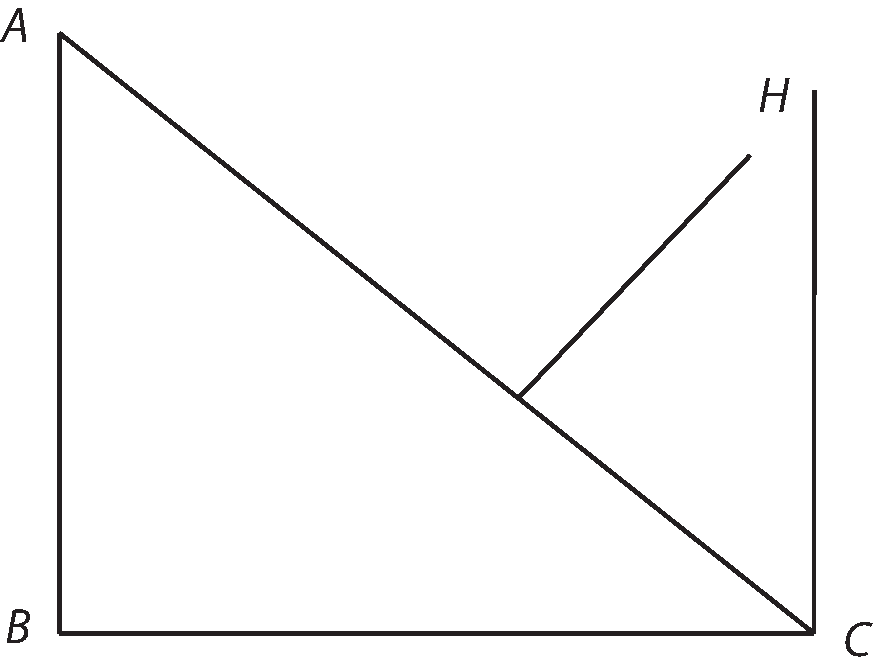
\includegraphics[width=0.83\textwidth]{images/LH037,03_86r-d1.pdf}
\end{minipage}
\hspace*{7mm}
\begin{minipage}[t]{0.5\textwidth}
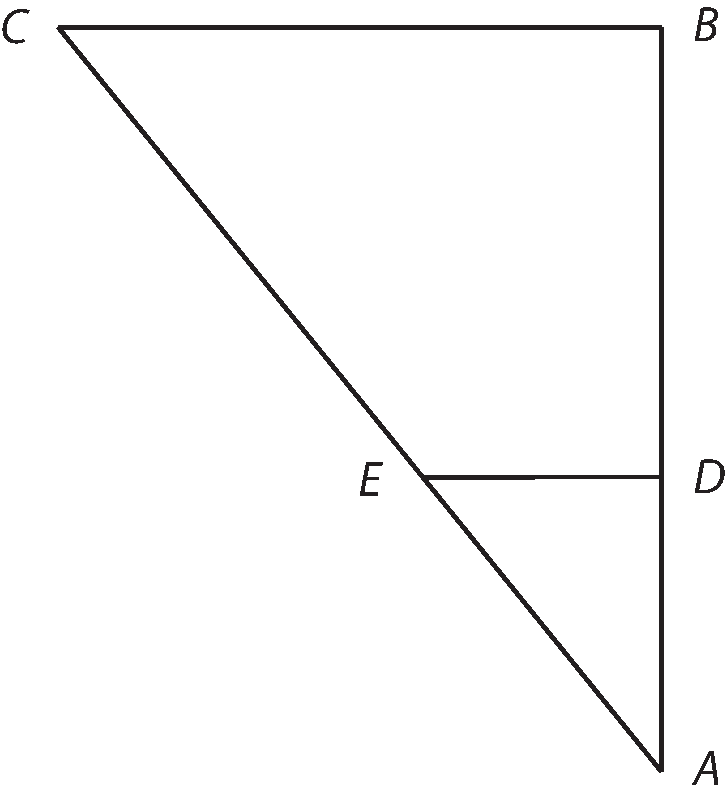
\includegraphics[width=0.67\textwidth]{images/LH037,03_86r-d2.pdf}
\end{minipage}
\pend
\count\Bfootins=1000
\pstart
%\vspace*{1mm}
\hspace{6.8mm} [\textit{Fig. 1, gestrichen}] \hspace*{45mm}  [\textit{Fig. 2, gestrichen}]
%\begin{minipage}[t]{0.2\textwidth}
%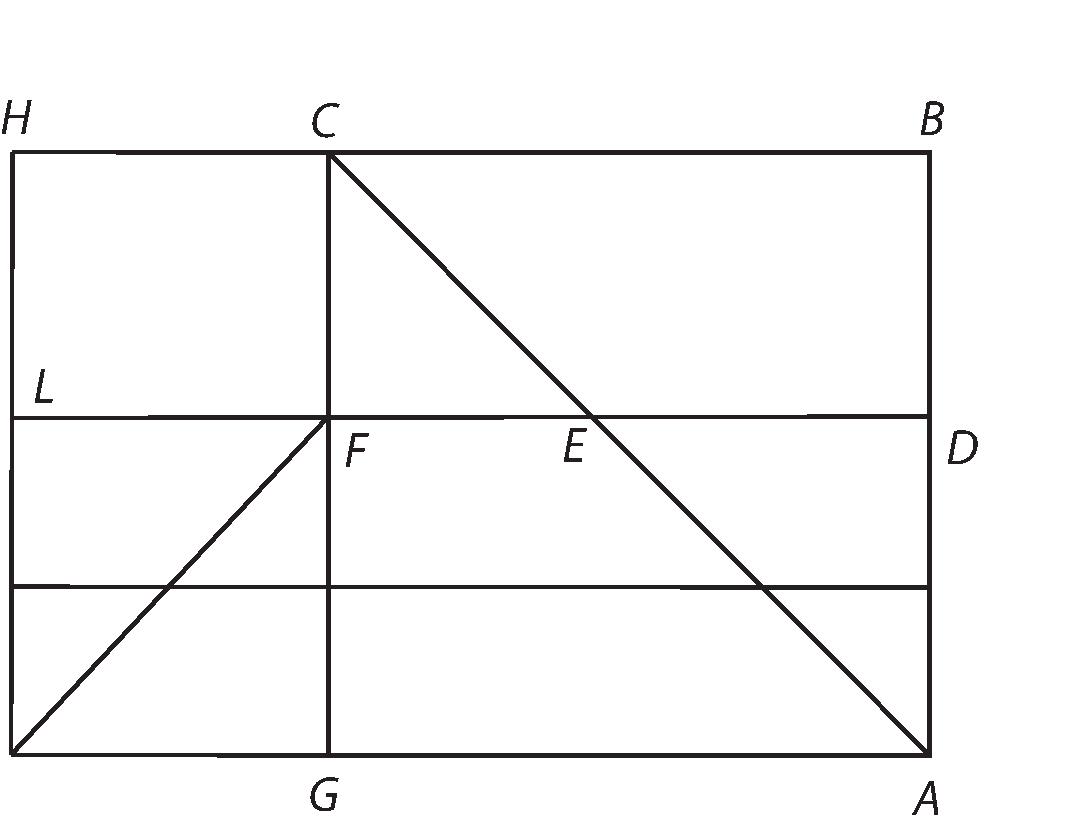
\includegraphics[width=1.5\textwidth]{images/LH037,03_86r-d3.pdf}
%\noindent \centering [\textit{Fig. 3}]
%\end{minipage}
%    \vspace*{5mm}
\pend 
\vspace{1.1em}
\pstart
\noindent Tout \setline{1}cela bien consideré, nous donnera les fondemens du calcul. Soit en premier lieu un \edtext{triangle, $ABC$ la hauteur $ADB$}{\lemma{triangle,}\Bfootnote{\textit{(1)}\ la hauteur de l'eau $ADB$, \textit{(a)} faisan \textit{(b)} alors faisant abstraction du frottement\protect\index{Sachverzeichnis}{frottement} \textit{(2)}\ $ABC$ la hauteur $ADB$, \textit{L}}}, et $DE$ ordonnée parallele à la base; je dis que $ADB$ estant aussi la hauteur de l'eau dont $A$ est le dessous, $B$ le \edtext{dessus, et $D$ un autre point quelconque du milieu, la vitesse}{\lemma{dessus,}\Bfootnote{\textit{(1)}\ la vistesse \textit{(2)}\ et $D$ [...] vitesse \textit{L}}} de l'eau en $D$ sera representée par l'ordonnée $DE$ \edtext{ou les vistesses seront comme les $DE$}{\lemma{ou les [...] les $DE$}\Bfootnote{\textit{erg. L}}} justement, comme croistroit la \edtext{vistesse d'une boule}{\lemma{vistesse}\Bfootnote{\textit{(1)}\ d'un morceau \textit{(2)}\ d'une piece \textit{(3)}\ d'une boule \textit{L}}} de bois,\hfill qui\hfill monteroit\hfill du\hfill fonds\hfill \edtext{en\hfill haut}{\lemma{en haut,}\Bfootnote{\textit{erg. L}}},\hfill par\hfill un\hfill mouvement\hfill  \edtext{acceleré.\hfill Par\hfill consequent}{\lemma{acceleré.}\Bfootnote{\textit{(1)}\ Faisons a \textit{(2)}\  Entrons à present plus avant dans la matiere, et faisons neantmoins abstraction de l'epaisseur de l'eau. \textit{(3)}\ Par consequent \textit{L}}}\hfill la\hfill 
\pend
\vspace{1.1em}
%\vspace{-10mm}
\pstart
\centering
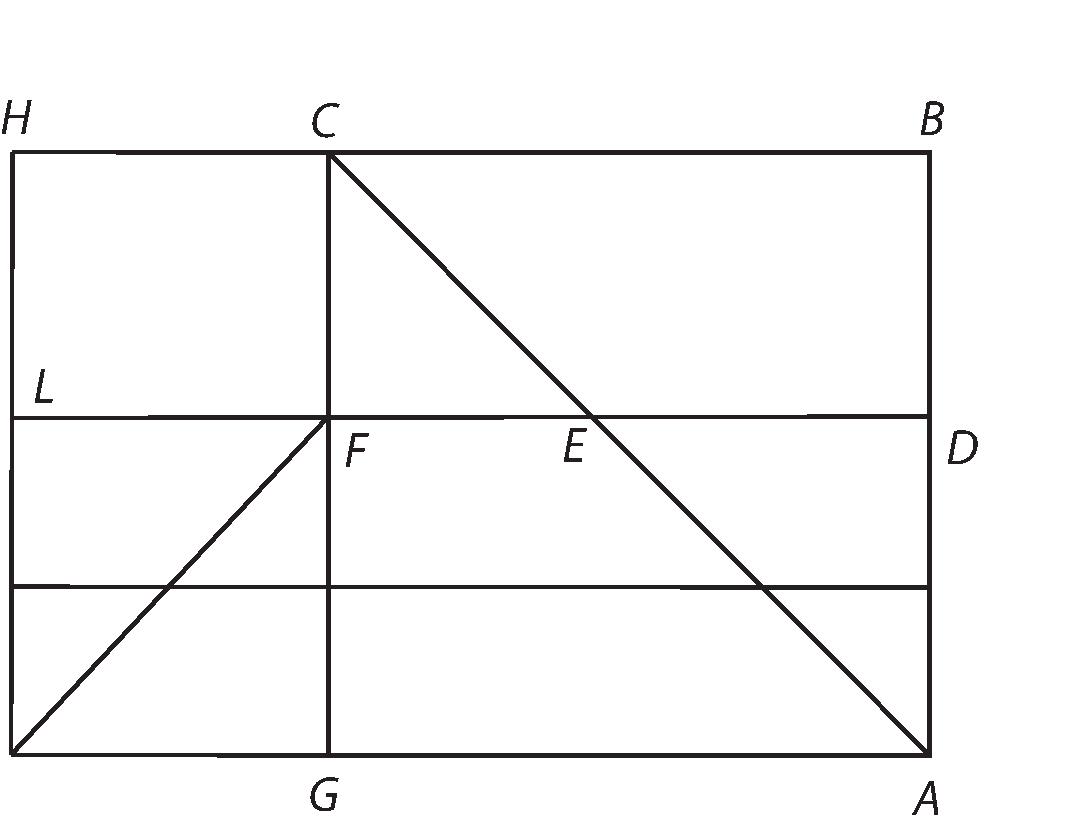
\includegraphics[trim = 0mm 0mm 0mm 0mm, clip,width=0.47\textwidth]{images/LH037,03_86r-d3.pdf}\\
\centering [\textit{Fig. 3}]
\pend
\newpage
\count\Bfootins=1200
\pstart
\centering
\includegraphics[trim = 0mm 0mm 0mm 0mm, clip, width=0.6\textwidth]{images/LH037,03_86r-d4.pdf}\\
 \noindent \centering [\textit{Fig. 4, gestrichen}]
\pend
\vspace{1.5em}
\pstart \noindent force \setline{1}de l'eau\protect\index{Sachverzeichnis}{eau} contre une digue, \edtext{seroit la moitié}{\lemma{seroit}\Bfootnote{\textit{(1)}\ le double \textit{(2)}\ la moitié \textit{L}}} de celle qu'exerceroit la m\^{e}me eau, si elle estoit par tout m\"{u}e d'une vistesse egale à celle de l'eau, d'en haut. Entrons plus avant en matiere, et faisons encor \edtext{abstraction de la largeur de la riviere, passons au frottement.\protect\index{Sachverzeichnis}{frottement}}%
{\lemma{abstraction}\Bfootnote{%
\textit{(1)}\ de l'épaisseur de l'eau, venons au frottement %
\textit{(2)}\ de la [...] frottement. \textit{L}}}
Il est manifeste, que l'eau qui est plus pressée tiendra plus contre son support, et coulera avec plus de difficulté là dessus.
Or celle qui est plus basse est plus pressée;
\edtext{donc accomplissant le $\square$le $ABCG$ je dis que}%
{{\lemma{donc}\Bfootnote{%
\textit{(1)}\ faisant un autre triangle $ABG$, de sorte que $CBG$ soit une %
\textit{(a)} droite %
\textit{(b)} m\^{e}me droite, et $EDF$ et $AFG$, de m\^{e}me lignes droites, je dis que %
\textit{(2)}\ accomplissant [...] dis que \textit{L}}}%
{\lemma{donc [...] je dis que}\Cfootnote{%
In der Textvariante \textit{(1)} bezieht sich Leibniz mit \glqq triangle $ABG$\grqq\ auf eine nachträglich gestrichene Variante von [\textit{Fig. 3}],
die hier als [\textit{Fig. 4}] wiedergegeben wird.}}}
les \edtext{pressions\protect\index{Sachverzeichnis}{pression} ou difficultés, que l'eau aura à glisser, dans les hauteurs comme $D,$}%
{\lemma{pressions}\Bfootnote{\textit{(1)}\ dans les hauteurs comm %
\textit{(2)}\ ou difficultés, [...] comme $D,$ \textit{L}}}
seront comme les ordonnées $EF$ du $\bigtriangleup$ $CGA$, ou complemens des $DE$. Il y a pourtant quelque chose à redire, car quoyque cela arriveroit des aix\protect\index{Sachverzeichnis}{aix} estant mis les uns sur les autres, et autres matieres solides, à cause qu'alors ce qui passe ouure les pores de l'autre, et
\edtext{l'accommode aux}{\lemma{l'accommode}\Bfootnote{\textbar\ aussi \textit{gestr.} \textbar\  aux \textit{L}}}
siens, d'o\`{u} vient cette liaison, et cette difficulté de trainer ou de glisser: neantmoins les liquides paroissent estre d'une autre nature. Car toute la pression\protect\index{Sachverzeichnis}{pression} est egalement distribuée. Cela pourtant ne me satisfait pas. Il est vray qu'une mouche ou chassée dans une grosse masse de fer, ou m\^{e}me paste ou sable n'en sera pas ecrasée; à cause que tout se soutient; neantmoins le plan tout entier sera tousjours pressé d'un plan superieur tout entier. Il s'agit donc seulement de s\c{c}avoir si cette pression\protect\index{Sachverzeichnis}{pression} rend l'eau basse pour ainsi dire plus gluante, et \edtext{moins aisée}{\lemma{moins}\Bfootnote{\textit{(1)}\ difficile \textit{(2)}\ aisée \textit{L}}}
 à separer. Mais cela ne se
[86~v\textsuperscript{o}]
remarque pas m\^{e}me  dans les eaux dormantes; car le frottement\protect\index{Sachverzeichnis}{frottement} vient de cette insertion mutuelle des eminences dans les pores; la quelle  apparement au moins demeure la m\^{e}me  dans l'eau haute ou basse. Neantmoins on pourra faire des experiences la dessus dans une  eau dormante; remuant l'eau d'en haut si elle emporte moins aisement avec elle celle qui est un pied au dessous d'elle, que l'eau d'en  bas, ou du milieu emporte celle qui est d'un pied au dessus elle. Item si l'eau emporte plus aisement celle qui est au dessous, que celle qui est  laterale, la distance estant \'{e}gale. Cela se peut experimenter dans les canaux, en suspendant certaines choses, en certains endroits. Quoyqu'il en  soit, faisant \edtext{abstraction de l'augmentation de l'adherence\protect\index{Sachverzeichnis}{adherence}, venant de la pesanteur}{\lemma{abstraction}\Bfootnote{\textit{(1)}\ de la pression \textit{(2)}\ de [...] pesanteur; \textit{L}}}; il est tousjours constant, \edtext{qu'une partie de l'eau}{\lemma{qu'une}\Bfootnote{\textit{(1)}\ eau \textit{(2)}\ partie de l'eau \textit{L}}} \edtext{remu\'{e}e communique}{\lemma{remu\'{e}e}\Bfootnote{\textit{(1)}\ propage \textit{(2)}\ communique \textit{L}}} son mouuement \`{a} celle qui est voisine, et cellecy encor \`{a} une autre voisine, que la vistesse diminue la matiere \`{a} remuer  estant augment\'{e}e. Et que celle qui est plus voisine est plus remu\'{e}e; parce que jamais celle qui est remu\'{e}e, suit parfaitement celle qui la  remue. Dont il est assez difficile de donner la raison. Posons plusieurs aix\protect\index{Sachverzeichnis}{aix} l'un sur l'autre. Tirons celui qui est au dessus, tous les autres suivront un peu,  plus ou moins selon le voisinage. Donc la raison est, soit une chose li\'{e}e \`{a} une corde\protect\index{Sachverzeichnis}{corde} qui se peut \edtext{\'{e}tendre, tirons la corde, le corps}{\lemma{\'{e}tendre,}\Bfootnote{\textit{(1)}\ la chose \textit{(2)}\ tirons la corde, le corps \textit{L}}}
%%
suivra un peu, mais il restera aussi un peu, selon que la corde se peut \'{e}tendre.
La glutinosit\'{e}\protect\index{Sachverzeichnis}{glutinosit\'{e}} ou adh\'{e}rence s'expliquera par une
%%
\edtext{telle}{\lemma{telle}\Bfootnote{\textit{erg. L}}}
%%
corde. Il se peut faire que la glutinosit\'{e}\protect\index{Sachverzeichnis}{glutinosit\'{e}} dans les liquides n'empeche pas le mouuement,
mais le retarde seulement, en augmentant la quantit\'{e} du mobile.
J'avois  commenc\'{e} \`{a}
\edtext{douter s'il}{\lemma{douter}\Bfootnote{\textit{(1)}\ si \textit{(2)}\ s'il \textit{L}}}
y auroit icy une composition du mouuement,\protect\index{Sachverzeichnis}{composition du mouuement}
\`{a} cause du support. Sur le plan inclin\'{e}
%%
\edtext{immobile}{\lemma{immobile}\Bfootnote{\textit{erg. L}}} \edtext{$AB$ glisse}{\lemma{$AB$}\Bfootnote{\textit{(1)}\ roule \textit{(2)}\ glisse \textit{L}}} l'aix\protect\index{Sachverzeichnis}{aix} $CD$ et sur celuy-cy l'aix\protect\index{Sachverzeichnis}{aix} $EF$. On dira que $CD$, et $EF$, estant port\'{e} par un m\^{e}me  principe glisseront tousjours de compagnie, et qu'il n'y a point de raison que $E$, s'eloigne \setline{21}de $C$. 
\pend
\pstart
\centering 
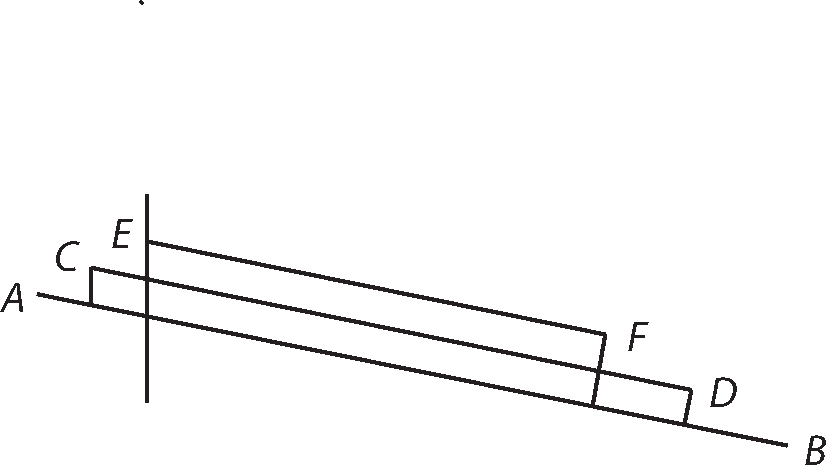
\includegraphics[trim = 0mm 0mm 0mm 18mm, clip,width=0.48\textwidth]{images/LH037,03_86v-d1.pdf}\\
 \noindent \centering [\textit{Fig. 5}]
\pend
\newpage
\pstart
\noindent Je reponds qu'il n'iront pas de compagnie, en voicy la raison. Posons que deux marteaux d'une force \'{e}gale, direction parallele \`{a} $AB$ frappent l'un in $C.$ l'autre in $E.$
je dis
\edtext{que l'effort\protect\index{Sachverzeichnis}{effort} du marteau inferieur in $C$ sera communiqu\'{e}}{\lemma{que}\Bfootnote{%
\textit{(1)}\ l'aix %
\textit{(2)}\ l'effort \textbar\ de l'un \textit{streicht Hrsg.} \textbar\ %
\textit{(a)}\ des marteaux sera commu %
\textit{(b)}\ du marteau [...] communiqu\'{e} \textit{L}}}
aussi \`{a} l'aix\protect\index{Sachverzeichnis}{aix} $EF$,
et qu'en m\^{e}me temps l'aix\protect\index{Sachverzeichnis}{aix} $EF$ estant
\edtext{frapp\'{e} d'un autre}{\lemma{frapp\'{e}}\Bfootnote{\textit{(1)}\ de deux \textit{(2)}\ d'un autre \textit{L}}}
marteau, sera port\'{e} par ces deux
\edtext{efforts. Mais la communication se fait selon adherence.\protect\index{Sachverzeichnis}{adherence}
La cheute d'un corps pesant}%
{\lemma{efforts.}\Bfootnote{\textit{(1)}\ Nota un corps pesant continu \textit{(2)}\ Mais [...] pesant \textit{L}}}
solide est telle, qu'une impression du liquide general sur une partie est aussi sur toutes  les autres,
\`{a} cause de la connexion; mais il ne va pas plus viste pour cela;
\`{a} cause que l'effect de l'impression est d'autant plus foible,
que  la matiere \`{a} emporter (movenda) est plus grande, la direction estant en $AB$,
une \edtext{ligne solide}{\lemma{ligne}\Bfootnote{\textit{(1)}\ rigide \textit{(2)}\ solide \textit{L}}}
$AB$ estant prise.
Il s'agit  de s\c{c}avoir si $AC$ fait impression sur $CB.$ Il semble que non.
Car \`{a} mesure que $AC$ entre dans la place de $CB$, $CB$ en sort.
\pend
\pstart
\begin{wrapfigure}[5]{l}{0.42\textwidth} 
\vspace{-4.5mm}\includegraphics[width=0.42\textwidth]{images/LH037,03_86v-d2.pdf}\\
 \noindent \centering [\textit{Fig. 6}]
\end{wrapfigure}
\noindent 
Mais  si nous le supposions; alors $ACB$ estant solide, \edtext{$CB$ emporteroit}{\lemma{$CB$}\Bfootnote{\textit{(1)}\ allant plus vis \textit{(2)}\ emporteroit \textit{L}}} de m\^{e}me $AC$ et tout reviendroit \`{a} la m\^{e}me  chose.  Mais si $ACB$ liquide parfaitement, il seroit dispers\'{e} en parties infiniment petites; si deux aix\protect\index{Sachverzeichnis}{aix} estoient parfaitement  \edtext{polis, pourroit-on}{\lemma{polis,}\Bfootnote{\textit{(1)}\ vous pourriez \textit{(2)}\ pourroit-on \textit{L}}} pousser celuy d'en bas sans que celuy d'en haut f\^{i}t effort de le suivre? Je \edtext{croy que celuy}{\lemma{croy}\Bfootnote{\textit{(1)}\ que non; et \textit{(2)}\ que celuy \textit{L}}} d'en  haut estant suppos\'{e} pesant, \edtext{suivra de m\^{e}me}{\lemma{suivra}\Bfootnote{\textit{(1)}\ sans doute \textit{(2)}\ de m\^{e}me  \textit{L}}} que ce qui est sur un aix\protect\index{Sachverzeichnis}{aix} qui flotte suit l'aix. Cela estant nous avons trouu\'{e} \edtext{la cause de l'union dans les corps.}{\lemma{}\Afootnote{\textit{Zwischen den Zeilen:} NB. Puto hoc non iri, ex praetensa minimorum penetratione, sed ob insinuationes partium.}} S\c{c}avoir deux corps sont unis l'un \`{a} l'autre; lors que l'un fait effort d'entrer dans la place de l'autre, pendant que l'autre fait effort d'y rester. On y reste effectivement.
Sed hoc obiter.
Difficultas, an haec unio sit reciproca?
Videtur.
Nihil enim refert huic an illi tribuas conatum approprinquationis\protect\index{Sachverzeichnis}{conatus approprinquationis}. Hinc sequitur in nostro casu aeque sequi conari aquam subjacentem motum superstantis, quam contra. Tantum discrimen ab eo  esse, quod ultima subjacentium a fundo plurimum retinetur. \edtext{Si adhaesioni\protect\index{Sachverzeichnis}{adhaesio}}{\lemma{Si}\Bfootnote{\textit{(1)}\ pressioni\protect\index{Sachverzeichnis}{pressio} \textit{(2)}\ adhaesioni\protect\index{Sachverzeichnis}{adhaesio} \textit{L}}} a pondere\protect\index{Sachverzeichnis}{pondus} ortae, \edtext{adjiciatur adhaesio\protect\index{Sachverzeichnis}{adhaesio} a pressione[,] tunc\protect\index{Sachverzeichnis}{pressio}}{\lemma{adjiciatur}\Bfootnote{\textit{(1)}\ pressio\protect\index{Sachverzeichnis}{pressio} orta \textit{(2)}\ adhaesio\protect\index{Sachverzeichnis}{adhaesio} a pressione[,]\protect\index{Sachverzeichnis}{pressio} \textit{L}}} ad $\triangle$lum $CGH$ addendo $\square$lum $GCH.$ cujus ordinata $LF.$
erunt adhaesiones\protect\index{Sachverzeichnis}{adhaesio} ut ordinatae $LFE.$
Si plures asseres sibi imponantur, in plano inclinato ut paulo ante dixi,
infimus tardius ibit, quam iret, si caeteri non adessent,
non tantum ob frictionem\protect\index{Sachverzeichnis}{frictio}
contra fundum seu planum inclinatum\protect\index{Sachverzeichnis}{planum inclinatum} immobile,
sed etiam ideo quia
\edtext{eo}{\lemma{eo}\Bfootnote{\textit{erg. L}}}
plura secum auferente aucta materia minui motus debet.
\edtext{Aqua subjacens}{\lemma{Aqua}\Bfootnote{\textit{(1)}\ superstans \textit{(2)}\ subjacens \textit{L}}}
videtur perfecte secum auferre superstantem, sed motu qui sit reciprocus quantitatum.
Nimirum sit conatus\protect\index{Sachverzeichnis}{conatus}
\edtext{[quo]}{\lemma{qua}\Bfootnote{\textit{L ändert Hrsg.}}}
punctum aqueum $A$ in plano inclinato\protect\index{Sachverzeichnis}{planum inclinatum}
libere progrederetur certus ut $\beta.$
erit totius lineae $AB$ conatus hoc primo conatu $\beta$ ablatae ad conatum\protect\index{Sachverzeichnis}{conatus} $\beta$,
ut punctum $A$, seu linea infinitesima, quam vocabimus $\varphi.$ est ad totam rectam $AB.$
eodem modo si sumatur punctum aqueum $D$ rursus $\sqcap\ \varphi.$
erit $\beth$ conatus\protect\index{Sachverzeichnis}{conatus} totius linea superstantis $AD$ ad $\beta$ conatum puncti aquei $D.$
ut $D$ est ad $AD$ seu ut ad $X.$ vocando $AD\, \sqcap\, X$.
Ergo summa omnium conatuum quos punctum aliquod accipit ab inferioribus omnibus,
exprimetur per quadraturam hyperbolae\protect\index{Sachverzeichnis}{hyperbola}\protect\index{Sachverzeichnis}{quadratura}
\edtext{seu logarithmos.\protect\index{Sachverzeichnis}{logarithmus} Sed}{\lemma{seu}\Bfootnote{%
\textit{(1)}\ summam %
\textit{(2)}\ logarithmos. %
\textit{(a)}\ Porro ista %
\textit{(b)}\ Sed \textit{L}}}
jam vicissim cogitandum:
inferiorem aquam proprio superioris conatu\protect\index{Sachverzeichnis}{conatus} auferri.
Eodem plane modo contrariam describendo Hyperbolam\protect\index{Sachverzeichnis}{hyperbola}
cujus quadratura opus est.
Unde si hic quoque conatus aeque ac primus effectum sortiretur suum,
summa atque ima aqua eodem modo moverentur, non vero intermediae.
Sed fundi immobilis renitentia turbat.
Quae jam consideranda est, scilicet fundi renitentia, cum sit infinita:
connexio inter fundum et aquam infimam dissolvetur necessario motu aquae,
et quia fundus ob resistentiam\protect\index{Sachverzeichnis}{resistentia} infinitam nihil supponetur accipere mutationis
(+~abstrahimus enim animum ab abrasionibus\protect\index{Sachverzeichnis}{abrasio}~+)
ideo tota superatio resistentis seu causae adhaesionis\protect\index{Sachverzeichnis}{adhaesio}
redundabit in ipsum motum aquae fundum radentis,
qui eo erit tardior, quo plus motus produxit in superando obstaculo.
Videndum an cohaesio\protect\index{Sachverzeichnis}{cohaesio} facta ob pressionem\protect\index{Sachverzeichnis}{pressio}
et ipsi pressioni\protect\index{Sachverzeichnis}{pressio} proportionalis.
Hoc definiendum experimentis,\protect\index{Sachverzeichnis}{experimentum}
ut si asseres sibi imponas, item chordis pondera\protect\index{Sachverzeichnis}{pondus} appendas,
et tractionem\protect\index{Sachverzeichnis}{tractio} examines.
Ponamus diminutiones unius superstantis esse ipsis $LF$ proportionales.
Conatus ergo imi [\textit{Text bricht ab.}]
\pend
\newpage
\count\Afootins=1500
\count\Bfootins=1500
\count\Cfootins=1500